Es el cambio de dirección que experimenta un onda cuando choca contra una superficie y regresa al medio del cual provenie. Las superficies planas y duras reflejan más. Esto ocurre con diversas ondas como luz, sonido y las ondas en la superficie del agua.

\begin{figure}[H]
  \centering
  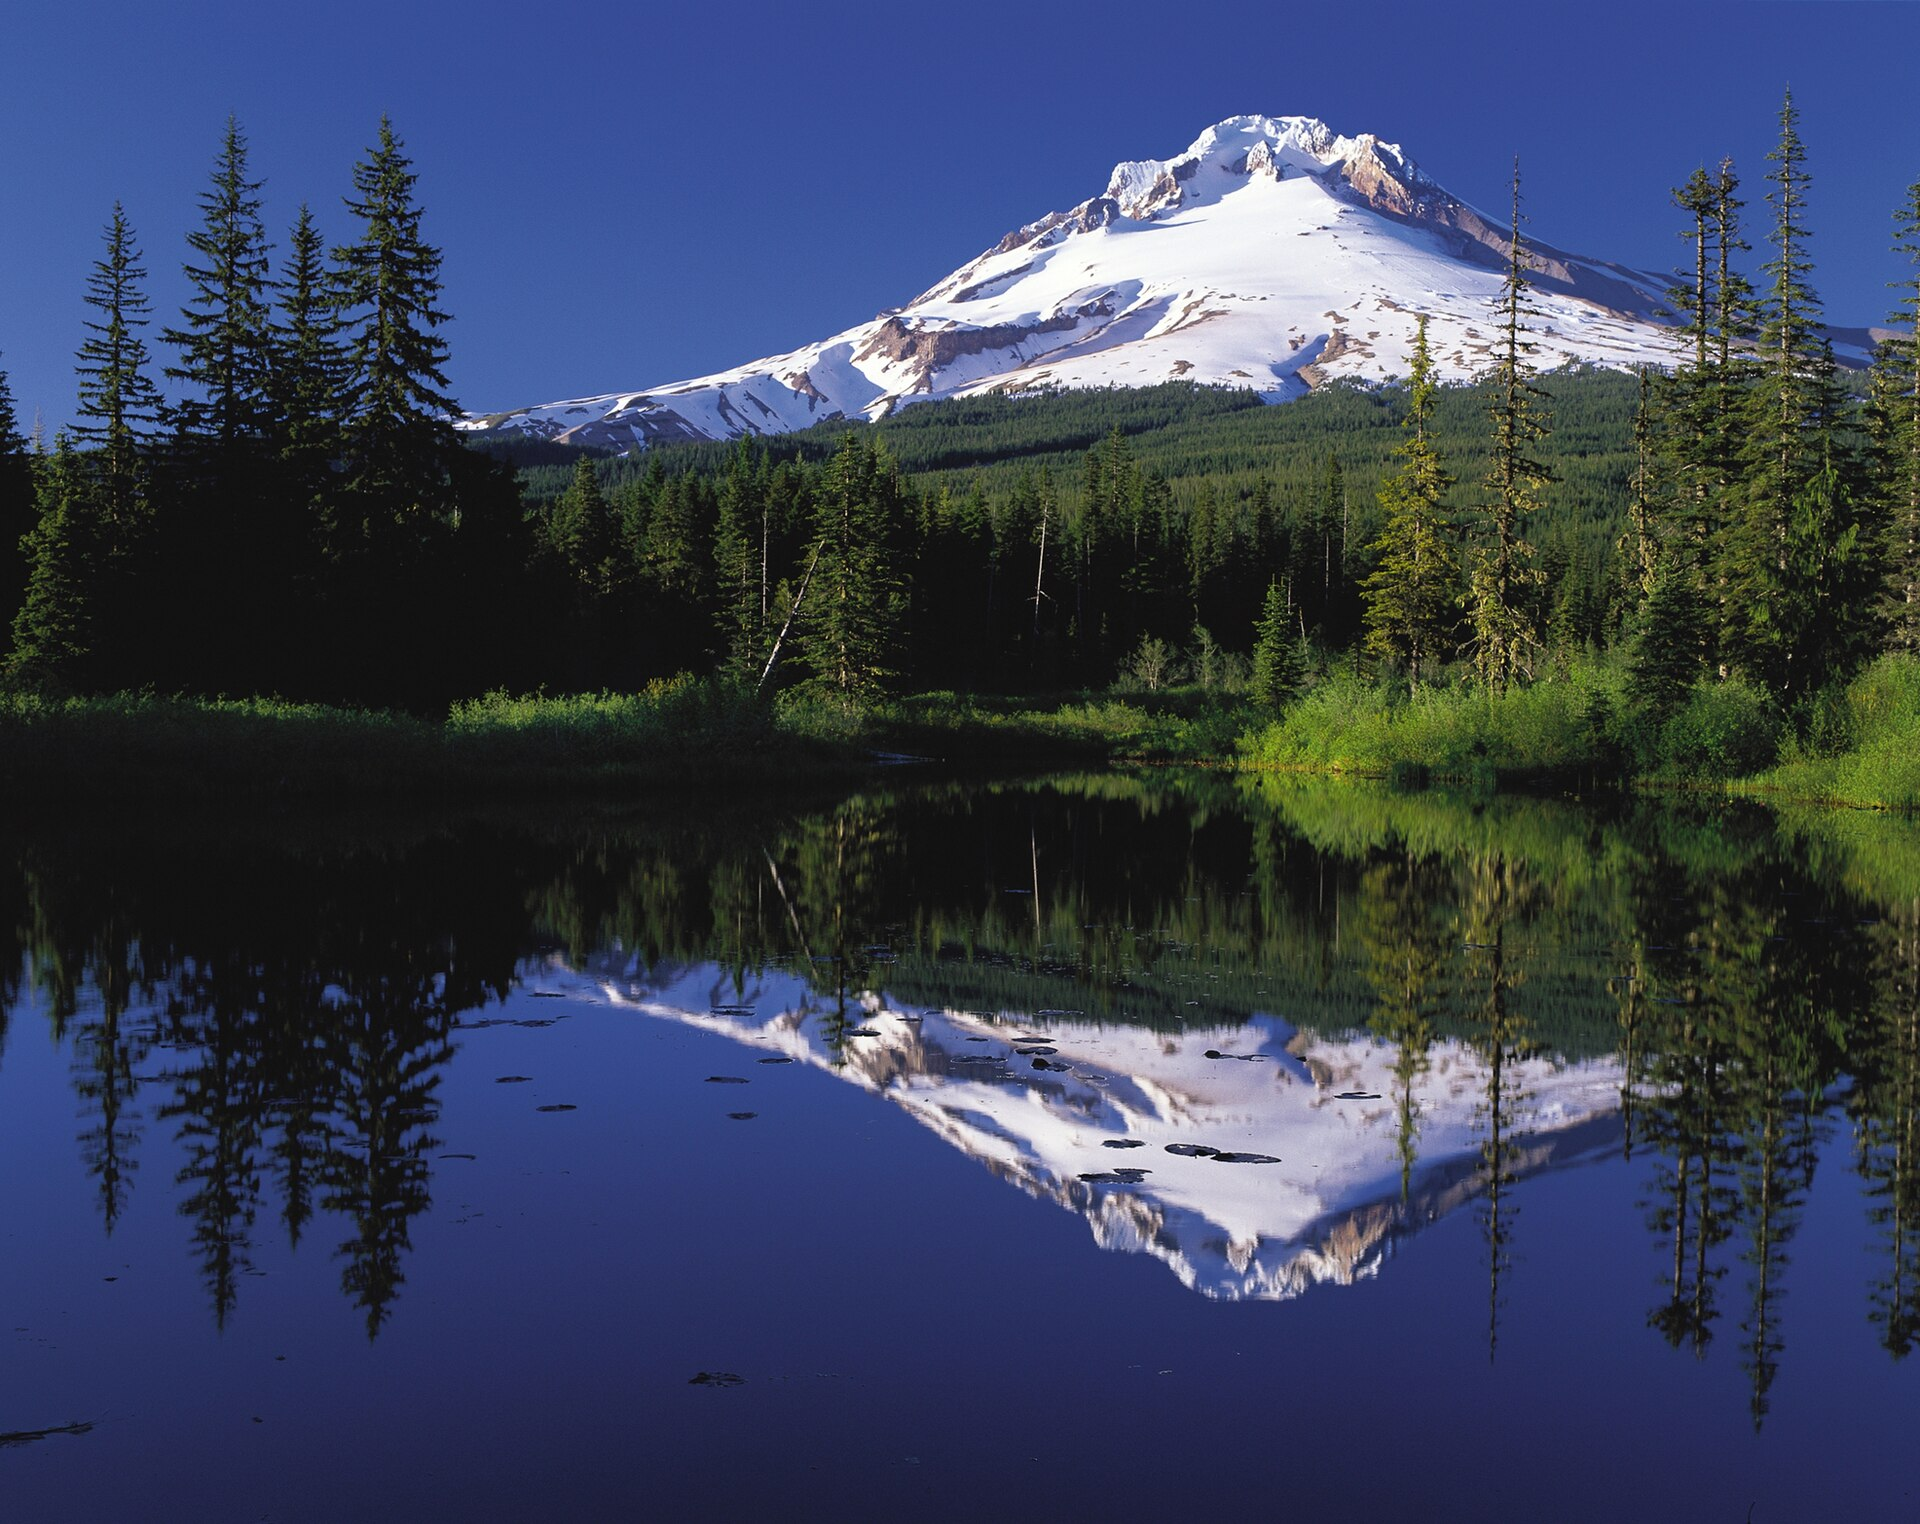
\includegraphics[scale=0.15]{imagenes/reflexion_monte.png}
  \caption{Reflexión en el agua\cite{wikireflexion}}
\end{figure}

El \textbf{eco} es un ejemplo de este fenómeno. Cuando una onda sonora choca contra una superficie, parte de la energía de la onda se refleja. Esto se percibe como un sonido distinto al original, debido a la separación temporal entre la onda emitida y reflejada. También se puede mencionar la \textbf{reverberación}, en este caso en un reflejo continuo de la onda de sonido.

La luz es otro caso preponderante. Toda la luz percibida por el ojo humano es el resultado de un rebote de las ondas de luz al chocar con multitud de superficies. Cuando el ojo no recibe ondas de luz, como en lugares oscuros o durante la noche, entonces percibe oscuridad. La luz de estrellas lejanas llega constantemente hasta el planeta tierra, aunque durante el día es opacada por la luz solar emitida por el sol ubicado en el centro del sistema solar donde se encuentra la tierra.
